% backup|Linear Algebra
% Add "% backup | [file name]" above (no quotes) to make file backup
\documentclass[12pt]{article}
% packages
\usepackage[paper=letterpaper,margin=2cm]{geometry}
\usepackage[skip=10pt plus1pt, indent=15pt]{parskip}
\usepackage{amsmath}
\usepackage{amssymb}
\usepackage{amsfonts}
\usepackage{graphicx}
\usepackage{titling}
\usepackage{subfig}
\usepackage{titleps}
\usepackage[x11names]{xcolor}
\colorlet{shadecolor}{LavenderBlush3}
\usepackage{delarray}
% \usepackage{framed}
\usepackage[colorlinks=true]{hyperref}


% settings
\setlength{\droptitle}{-6em}

\newpagestyle{mypage}{%
  \headrule
  \sethead{\MakeUppercase{}}{\textcolor{gray}{\thesubsection: \subsectiontitle}}{}
  \setfoot{}{\textcolor{gray}{\thepage}}{}
}

\pagestyle{mypage}

% \title{Linear Algebra}
% \author{Louis Meunier}
% \date{\textit{October 1, 2022 - ?}}

\begin{document}
% commands
\newcommand{\red}[1]{\textcolor{red}{#1}}
\newcommand{\ddx}{\frac{d}{dx}}
\newcommand{\ddy}{\frac{d}{dy}}
\newcommand{\dxdy}{\frac{dx}{dy}}
\newcommand{\dydx}{\frac{dy}{dx}}

\newcommand{\real}{\mathbb{R}}
\newcommand{\naturals}{\mathbb{N}}
\newcommand{\integers}{\mathbb{Z}}
\newcommand{\rational}{\mathbb{Q}}
\newcommand{\complex}{\mathbb{C}}

\newcommand{\twodmatrix}[2]{\begin{bmatrix}
#1\\
#2\\
\end{bmatrix}}
\newcommand{\twobytwomatrix}[4]{\begin{bmatrix}
#1 &#2\\
#3 &#4\\
\end{bmatrix}}

\hypersetup{
    linkcolor=violet
}

\begin{titlepage}
    \begin{center}
        \vspace*{1cm}
        \Huge
        \textbf{Linear Algebra and Geometry}
        
        \vfill
        
        \begin{figure}[!ht]
            \centering
            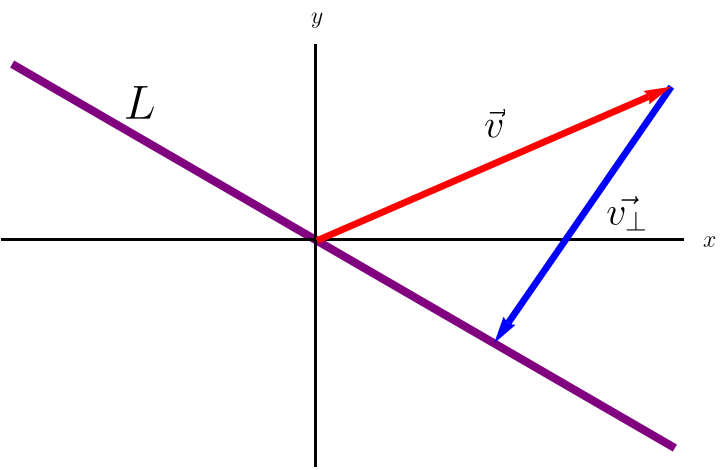
\includegraphics{misc/titlepage.png}
        \end{figure}
        \vfill
        
        \small
        by Louis Meunier
        
        \href{https://notes.louismeunier.net}{\color{violet}{notes.louismeunier.net}}
        
    \end{center}
\end{titlepage}


{
  \hypersetup{linkcolor=violet}
  \tableofcontents
}

\newpage
\section{Unit I}
\subsection{Solving Linear Systems}
\subsubsection{Algebraically vs Geometrically}
Consider a set of linear equations, $a_1 x+b_1 y = c_1$ and $a_1 x+b_2 y = c_2$. Solving this should be fairly straightforward:
\begin{itemize}
    \item Isolate one variable in one of the equations
    \item Substitute said variable in the second equation
    \item Solve for second variable
    \item Plug in solution to second variable in either original equation to find the other variable
\end{itemize}

Doing this reveals one of two things: either the system is consistent, or inconsistent:

\begin{itemize}\label{list:solntypes}
    \item \textbf{Consistent}: a solution to the system exists. This can either be:
    \begin{itemize}
        \item \textbf{A unique solution} (Fig. \ref{fig:uniquesolutions})
        \item \textbf{Infinite solutions} (Fig. \ref{fig:infinitesolutions})
    \end{itemize}
    \item \textbf{Inconsistent}: no solution to the system exists (Fig. \ref{fig:nosolutions})
\end{itemize}

Being able to recognize when these particular circumstances occurs is essential.

Graphically, the differences between these are also very noticeable (see figures  \ref{fig:uniquesolutions}, \ref{fig:infinitesolutions}, and \ref{fig:nosolutions}.)

\begin{figure}[!ht]%
    \centering
    \subfloat[\centering Two equations with a unique solution]{{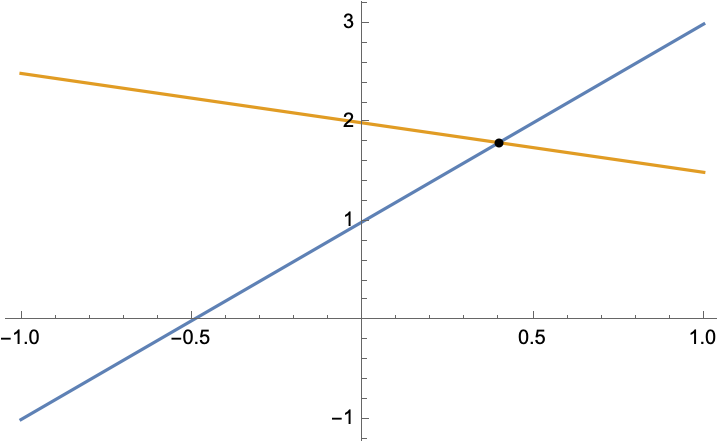
\includegraphics[width=6.5cm]{misc/twoequationsuniquesolution.png} }}%
    \qquad
    \subfloat[\centering Three equations with a unique solution]{{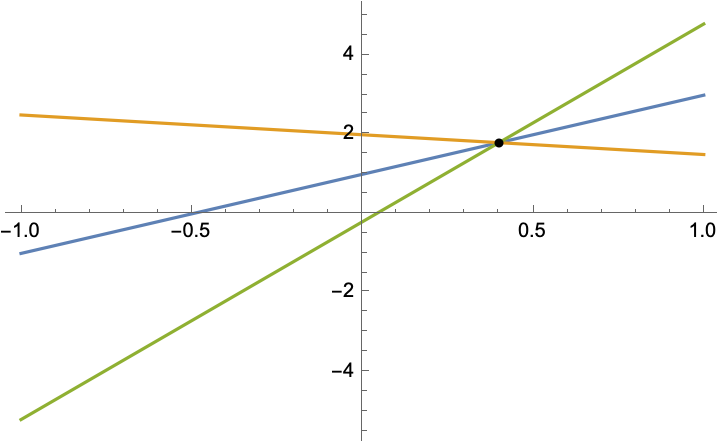
\includegraphics[width=6.5cm]{misc/threeequationsuniquesolution.png} }}%
    \caption{Unique solutions}
    \label{fig:uniquesolutions}%
\end{figure}

\begin{figure}[!ht]
    \centering
    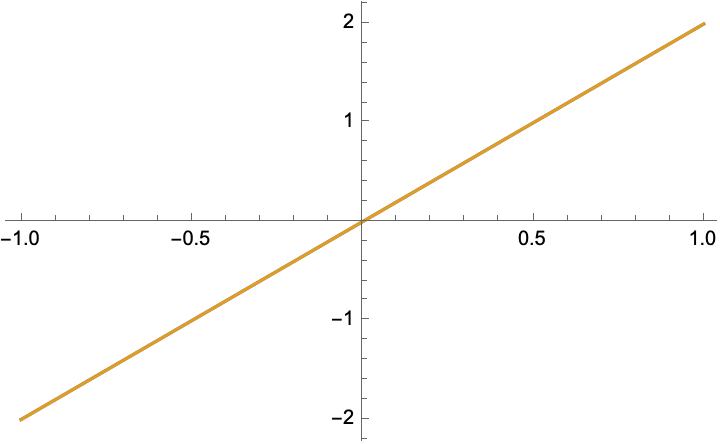
\includegraphics[width=6.5cm]{misc/infinitesolutions.png}
    \caption{Any number of equations with infinite solutions (always intersecting)}
    \label{fig:infinitesolutions}
\end{figure}

\begin{figure}[!ht]%
    \centering
    \subfloat[\centering Two equations with no solution]{{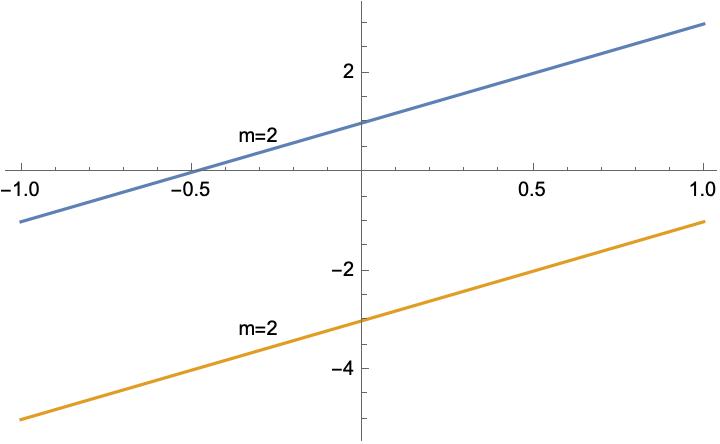
\includegraphics[width=6.5cm]{misc/twoequationsnosolution.png} }}%
    \qquad
    \subfloat[\centering Three equations with no solution]{{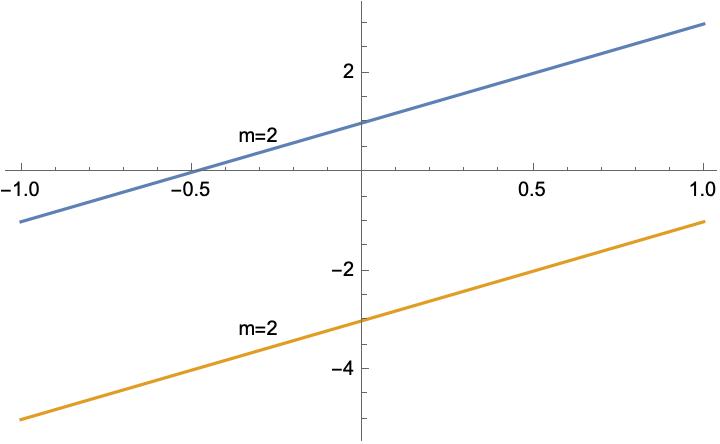
\includegraphics[width=6.5cm]{misc/twoequationsnosolution.png} }}%
    \caption{No solutions}
    \label{fig:nosolutions}%
\end{figure}

\subsubsection{Gaussian Elimination}
Although the procedure described above is fine for smaller equations, it can often become cumbersome. Using the concept of Gaussian Elimination, you can not only more easily solve systems of linear equations, but also determine patterns in said systems more easily.

To begin, create an \textbf{augmented matrix} of the system. This involves a \textbf{coefficient matrix} on the left, and the augmented part on the right.

The \textbf{coefficient matrix} has a row representing each equation, and each column representing the coefficients belonging to each individual variable in the system.

The \textbf{augmented matrix} contains each of the corresponding constants that the rows sum up to.

For example, the system

\begin{equation}
\begin{split}
    x + 2y - z &= 1\\    
    2x -3y + z &= 4\\
    y + 2z &= 0\\
\end{split}
\end{equation}

becomes

\[
    \begin{array}[t][{@{}ccc|c@{}}]
     1 & 2 & -1 & 1 \\
     2 & -3 & 1 & 4 \\
     0 & 1 & 2 & 0 \\
    \end{array}\
\]

Note that even though there is no $x$ in the third equation, its coefficient must still be represented (as a 0).

\subsubsection{rref}
When working with augmented matrices, there are a number of possible operations that can be used to reach the "end goal": \textbf{the row reduced echelon form (rref)}. An rref is achieved when:

\begin{itemize}
    \item The first non-zero term in each row (aka the \textbf{leading 1}) is a 1, and there are zeroes above and below it.
    \item The leading 1 in any row is to the right of the leading 1 above (\textit{this creates the typical staircase form}).
    \item Any rows with all zeros in the coefficient matrix are at the bottom.
\end{itemize}

A (very simple) rref matrix could look like this:

\[
    \begin{array}[t][{@{}ccc|c@{}}]
     1 & 0 & 0 & 1 \\
     0 & 1 & 0 & 4 \\
     0 & 0 & 1 & 0 \\
    \end{array}\
\]

To be clear: not all matrices will result in a nice, orderly pattern as this; most won't.

To get to this point at all, you must manipulate the matrix using certain operations:

\begin{itemize}
    \item Switch rows
    \item Add a multiple of one row to another
    \item Multiply a row by a constant
\end{itemize}

Note that all of these operations work on rows; attempting to manipulate columns will result in a wrong answer. 

\subsubsection{Determining Solutions from rref}

Given any rref matrix, you should be able to tell how many solutions a system has (and, by extension, what they are). The following examples should reveal some patterns in determining the number of solutions for any matrix:

\begin{itemize}
    \item 
    $
    \begin{array}[t][{@{}ccc|c@{}}]
     1 & 0 & 0 & c_1 \\
     0 & 1 & 0 & c_2 \\
     0 & 0 & 1 & c_3 \\
    \end{array}\
    $
    
    This system has \textbf{one unique solution}: when $x = c_1, y = c_2$ and $z = c_3$. This comes from the fact that each column represents a variable; thus, you can read the first row as $1*x+0*y+0*z = c_1$. The same idea applies for the rest of the rows.
    \item 
    $
    \begin{array}[t][{@{}ccc|c@{}}]
     1 & 0 & 0 & c_1 \\
     0 & 1 & 0 & c_2 \\
     0 & 0 & 0 & c_3 \neq 0 \\
    \end{array}\
    $
    
    This system has \textbf{no solutions}: in the final row is stating that $0*x+0*y+0*z \neq 0$, which is impossible. Thus, no solution to the system exists that would fulfil this requirement.
    \item 
    $
    \begin{array}[t][{@{}ccc|c@{}}]
     1 & 0 & 0 & c_1 \\
     0 & 1 & 0 & c_2 \\
     0 & 0 & 0 & 0 \\
    \end{array}\
    $
    
    This system has \textbf{infinite solutions}: in now row is there any restriction on the value of $z$. Thus, while $x = c_1$ and $y = c_2$, $z$ can be any real number. When this happens, $z$ is called a \textbf{"free variable"}. 
     
    In rref matrices of the following form, you can also have variables that are reliant on the value of free variables. 
     
     $$
    \begin{array}[t][{@{}ccc|c@{}}]
     1 & 0 & 0 & c_1 \\
     0 & 1 & 1 & c_2 \\
     0 & 0 & 0 & 0 \\
    \end{array}\
    $$
    
    In this case, $x = c_1$ and $y = c_2 - z$, where $z$ is free. It should be noted that you could also rewrite this as $z = c_2 - y$, in which case $y$ would be the free variable. Either way of writing it, there is one free variable.
\end{itemize}

There are many other forms, of varying complexity, that rrefs can have as well. However, following these simple patterns will make it fairly straightforward to determine the solutions in any situation.

\subsubsection{Representing Solutions}

As above, you can write the solutions to a system as $x = ..., y = ..., z = ...$. However, a more "standard" way, which will also make certain manipulations easier later, is:

\[
    \begin{bmatrix}
     x \\
     y \\
     z \\
    \end{bmatrix} 
    = 
    \begin{bmatrix}
     c_1 \\
     c_2 \\
     c_3 \\
    \end{bmatrix}
\]

Or, if there is a free variable: 
\[
    \begin{bmatrix}
    x \\
    y \\ 
    z \\
    \end{bmatrix}
    = 
    \begin{bmatrix}
    c_1 \\
    c_2 \\
    t \\
    \end{bmatrix}
    , t \in \real
\]

\subsubsection{Rank}

The \textbf{rank} of a matrix is the number of leading ones in the rref of that matrix. You can similarly say that the rank is equal to the number of columns of that matrix minus the number of free variables (though this way of thinking is more relevant later).

If a matrix has a rank equal to its number of columns, then the system of equations it represents is consistent and has a unique solution.

\subsection{Spans}
Before proceeding, we need to define a few concepts to analyze solutions and describe vectors and matrices in new ways.

A \textbf{linear combination} of the vectors $\Vec{v_1}, \Vec{v_2}, ..., \Vec{v_n}$ is an expression $c_1 \Vec{v_1} + c_2 \Vec{v_2} + ... + c_n \Vec{v_n}$, where $c_1, c_2,...,c_n \in \real$. In "simpler" terms, it is a sum of multiples of the vectors involved. 

A \textbf{span} of vectors is all possible linear combinations of a set of vectors, represented by the notation $span(\Vec{v_1}, \Vec{v_2}, ..., \Vec{v_n})$.

Spans can also be rewritten as a set; $span(\Vec{v_1}, \Vec{v_2}) = {c_1 \Vec{v_1} + c_2 \Vec{v_2}, c_1, c_2 \in \real}$. Being able to switch between these two forms will be important for later. 

Another important concept is being able to determine if a vector exists in a particular span; say, does the vector $\Vec{v}$ exist in $span(\Vec{x}, \Vec{y})$? This is the equivalent of asking whether a particular vector can be reached by summing multiples of a set of other vectors. Based on our "alternative" form of writing a span, we can say:

$$
\Vec{v} \stackrel{?}{\in} span(\Vec{x}, \Vec{y})={c_1\Vec{x} + c_2\Vec{y}, c_1,c_2 \in \real}
$$

Thus, we can say $\Vec{v} = c_1 \Vec{x} + c_2 \Vec{y}$. If and only if $c_1$ and $c_2$ exist can we say that $\Vec{v}$ is in $span(\Vec{x}, \Vec{y})$.


\subsection{Linear Relations}
Piggybacking off the ideas of linear combinations earlier, we can define a \textbf{linear relation} of vectors $\Vec{v_1}, \Vec{v_2}, ..., \Vec{v_n}$ as an equation of the form $c_1 \Vec{v_1} + c_2 \Vec{v_2} + ... + c_n \Vec{v_n} = \Vec{0}$.

If you can solve this equation where at least on $c_n$ is \textit{N
OT} 0, then this is called a \textbf{non-trivial linear relation}. Otherwise, if the only possible solution occurs when all $c_n$'s are 0, then this is a \textbf{trivial linear relation}.

From this, we can state yet another definition to describe vectors; \textit{linear (in)dependence}. A set of vectors can be described as \textbf{linearly independent} if the only linear relation between them that exists is the trivial one; conversely, a set of vectors are \textbf{linearly dependent} if a non-trivial linear relation exists.

Its helpful to think about this logically: if a set of vectors are \textit{dependent}, then one (or more) of the vectors relies on the one (or more) of the others. In more "mathematical" terms, this means that vectors in the set can be created from a sum of different multiples of others vectors in said set. This, on the other hand, is impossible between \textit{independent} vectors.

For example: is the vector $\begin{bmatrix}
1\\
2\\
\end{bmatrix}$ in $span(\begin{bmatrix}
-4\\
-5
\end{bmatrix}, \begin{bmatrix}
1\\
1\\
\end{bmatrix})$? If this were true, then we should be able to say that:

$$c_1 \twodmatrix{1}{1} + c_2 \twodmatrix{-4}{-5} = \twodmatrix{1}{2}, c_1, c_2 \in \real$$

$c_1$ and $c_2$ are, clearly, just \textit{scalars} of their respective vectors. As such, we can rewrite:

\begin{equation}
    \begin{split}
        \twodmatrix{c_1}{c_1} + \twodmatrix{-4 c_2}{-5 c_2} &= \twodmatrix{1}{2}\\
        \twodmatrix{c_1 - 4 c_2}{c_1 - 5 c_2} &= \twodmatrix{1}{2}
    \end{split}
\end{equation}

It should (hopefully) be clear that this is simply a system of linear equations, where $c_1$ and $c_2$ are the unknowns!

$$c_1 - 4 c_2 = 1; c_1 - 5 c_2 = 2$$

From here, we can simply use Gaussian elimination to see whether or not a solution does exist:

\[
    \begin{array}[t][{@{}cc|c@{}}]
     1 & -4 & 1 \\
     1 & -5 & 2 \\
    \end{array}\
    \Rightarrow
    \begin{array}[t][{@{}cc|c@{}}]
     1 & 0 & -3 \\
     0 & 1 & -1 \\
    \end{array}\
\]

Therefore, $c_1 = -3$ and $c_2 = -1$; as this system is consistent, then the vector is indeed in the span.

When working with spans of a number of vectors, it is important to be able to rewrite spans with as few vectors as possible; this is called the \textbf{basis} of the set. With more notation, we can say that the vectors $v_1, v_2, ..., v_n$ of set $V$ are a \textit{basis} of $V$ if they both \textit{span} $V$ and are \textit{linearly independent}. 

The first requirement here should make intuitive sense; if a set of vectors doesn't span $V$, then of course it can't represent it fully. 
The second requirement takes care of the "as few vectors as possible" part; if the opposite were true, and the vectors were linearly dependent, then one or more of the vectors could be represented by vectors already existing in the set.

Using the basis, we can then define the \textbf{dimension} of a set; the number of vectors in the \textit{basis} of the set.


\subsection{Subspaces}

A \textbf{subspace} of $\real^N$ is a non-empty set of vectors in $\real^N$, that can be described as a span of vectors. These two terms can often be interchanged, but be careful when you do so.

Formally, a subspace, $V$, must have the following properties:

\begin{enumerate}
    \item \textbf{Closed under scalar multiplication:} if $\Vec{u} \in V$, then $k\Vec{u} \in V$ for any scalar $k \in \real$ 
    \item \textbf{Closed under addition:} if $\Vec{v}, \Vec{w} \in V$, then $\Vec{v} + \Vec{w} \in V$.
\end{enumerate}

The concepts of bases and dimension similarly apply to subspaces, with the same rules.

\subsection{Standard Basis Vectors}
The standard basis vectors of $\real^n$ are written as $\Vec{e_i}$, with $i$ from $1$ to $n$, where the vector is made up of all 0's and a $1$ in the $i$th row. For example, the standard basis vectors $\real^2$ are $\Vec{e_1} = \twodmatrix{1}{0}, \Vec{e_2} = \twodmatrix{0}{1}$.

These standard basis vectors are, hopefully clearly, linearly independent; that is why they are called the "basis" after all. They will be helpful to use later on.

\subsection{Matrix-Vector Multiplication}
Being able to multiple a matrix by a vector has a large number of applications that are important to understand. We can approach defining matrix multiplication in a few ways.

\subsubsection{Column View}
Given a matrix $A$ and a vector $\Vec{x}$:

\[
A\Vec{x} = \begin{bmatrix}
&| &| & &|\\
&\Vec{c_1} &\Vec{c_2} &... &\Vec{c_n}\\
&| &| & &|\\
\end{bmatrix}\begin{bmatrix}
x_1\\
x_2\\
...\\
x_n\\
\end{bmatrix}=x_1 \Vec{c_1} + x_2 \Vec{c_2} + ... + x_n \Vec{c_n}
\]
 
In other words, this is defining the product of a matrix and vector as a linear combination of the columns of the matrix. It should be noted that this works by treating each column of the matrix $A$ as a vector; this can be helpful in better visualizing this operation.

\subsubsection{Row View}
Given a matrix $A$ and a vector $\Vec{x}$:

\[
A\Vec{x} = \begin{bmatrix}
&- & \Vec{r_1} &-\\
&- & \Vec{r_2} &-\\
& & ... &\\
&- & \Vec{r_m} &-\\
\end{bmatrix}\Vec{x}=\begin{bmatrix}
\Vec{r_1} \cdot \Vec{x}\\
\Vec{r_2} \cdot \Vec{x}\\
...\\
\Vec{r_m} \cdot \Vec{x}\\
\end{bmatrix}
\]

Note that "$\cdot$" represents a \textit{dot product}: this is the operation involving multiplying each element in one vector by the corresponding element in another vector.

Note that, conversely to above, this way of viewing the operation involves treating each row of $A$ as an individual matrix.

Deciding which "view" to use when is, often, very subjective to the particular situation. However, it should be noted that \textit{the result is the same no matter which view you take.}

\subsection{Linear Transformations}
A \textbf{linear transformation} $T: \real^n \to \real^m$ is a function that:
\begin{enumerate}
    \item \textbf{preserves vector addition}: $T(\Vec{x}+\Vec{y}) = T(\Vec{x}) + T(\Vec{y})$ for all $\Vec{x}, \Vec{y}$
    \item \textbf{preserves scalar addition}: $T(c \Vec{x}) = c T(\Vec{x})$ for all $\Vec{x}$ and $c \in \real$
\end{enumerate}

Linear transformations are often described by a matrix $A$, which \textit{induces} said linear transformation. In other terms:

\[
T: \real^n \to \real^m = T(\Vec{x}) = A\Vec{x}
\]

This matrix $A$ must be an $m$ x $n$ matrix in order for this formula to make sense.

\subsubsection{Determining Linear Transformations}
In order to figure out the linear transformation $T$ of any vector, you must know the $T(\Vec{x})$ of as many linearly independent $\Vec{x}$'s as there are columns in the matrix $A$. If you know, or are able to determine, the $T$ of the standard basis vectors of $A$, it is far easier to determine the linear transformation of any vector, thanks to the properties of linear transformations:
\[
T(\Vec{x}) = T(c_1 \Vec{e_1} + c_2 \Vec{e_2} + ...) = c_1 T(\Vec{e_1}) + c_2 T(\Vec{e_2}) + ...
\]

Using this same pattern, we can rewrite the $T$ of any vector $\Vec{x}$ as a sum of multiples of the $T$ of the standard basis vectors. 

\subsubsection{Geometric Linear Transformations}
Linear transformations can be visualized as a number of geometrical transformations; representing these in two dimensions makes it easiest to comprehend, but the same concepts are applicable to an arbitrary number of dimensions.

Say $T(\Vec{x}) = A\Vec{x}$, consider the following transformations on the standard basis vectors $\Vec{e_1}$ and $\Vec{e_2}$ of $\real^2$ (see figure \ref{fig:beforetransform}):

\begin{figure}[!ht]
    \centering
    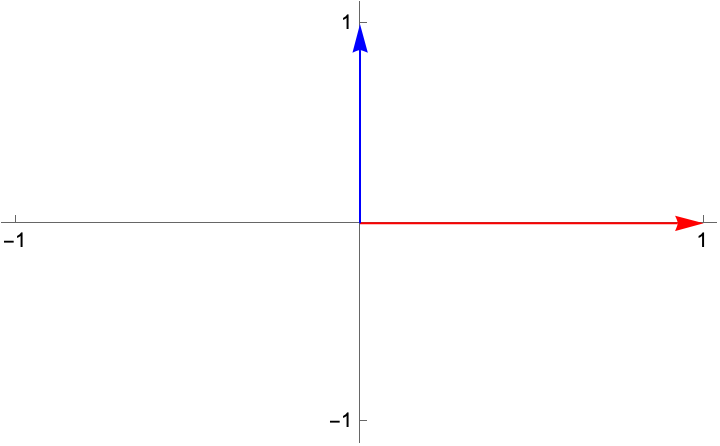
\includegraphics[width=8cm]{misc/beforetransformation.png}
    \caption{$\Vec{e_1}, \Vec{e_2}$ before any transformation}
    \label{fig:beforetransform}
\end{figure}
\newpage
\begin{itemize}
    \item $A = \begin{bmatrix}
    -1 &0\\
    0 &1\\
    \end{bmatrix}$ 
    
    $T(\Vec{e_1}) = \twodmatrix{1}{0} \twobytwomatrix{-1}{0}{0}{1} = \twodmatrix{-1}{0}, T(\Vec{e_2}) = \twodmatrix{0}{1} \twobytwomatrix{-1}{0}{0}{1} = \twodmatrix{0}{1}$
    
    \begin{figure}[!ht]
        \centering
        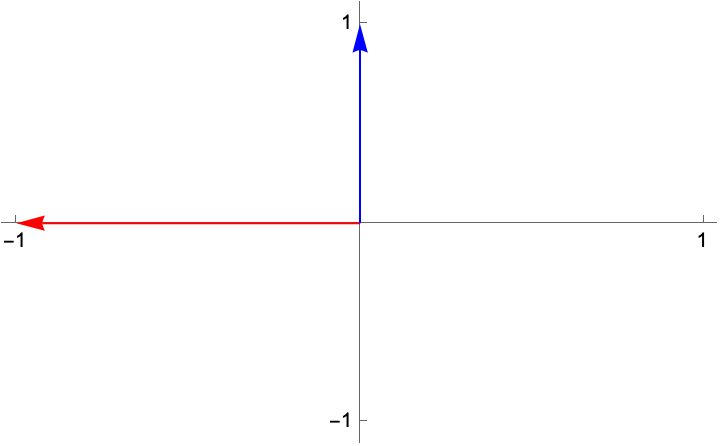
\includegraphics[width=8cm]{misc/reflectionoveryaxis.png}
        \caption{Reflection of $\Vec{e_1}, \Vec{e_2}$ over the y-axis}
    \end{figure}
    
    \item $A = \twobytwomatrix{0}{1}{1}{0}$ 
    
    $T(\Vec{e_1}) = \twodmatrix{1}{0} \twobytwomatrix{0}{1}{1}{0} = \twodmatrix{0}{1}, T(\Vec{e_2}) = \twodmatrix{0}{1} \twobytwomatrix{0}{1}{1}{0} = \twodmatrix{1}{0}$
    
    \begin{figure}[!ht]
        \centering
        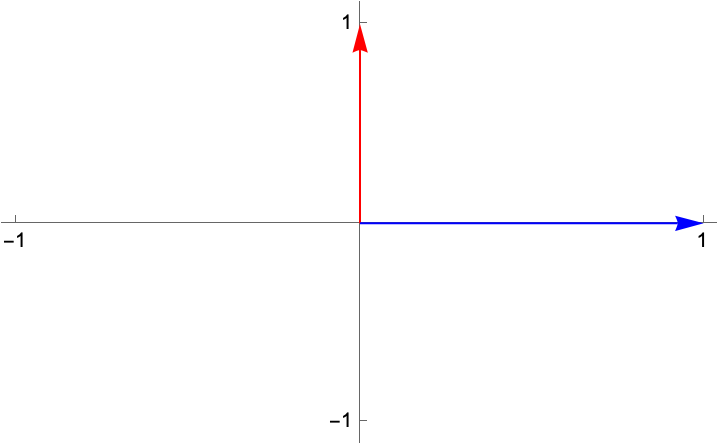
\includegraphics[width=8cm]{misc/reflectionoveryequalsx.png}
        \caption{Reflection of $\Vec{e_1}, \Vec{e_2}$ over $y=x$}
    \end{figure}
    \newpage
    \item $A = \twobytwomatrix{1}{-1}{0}{1}$ 
    
    $T(\Vec{e_1}) = \twodmatrix{1}{0} \twobytwomatrix{1}{-1}{0}{1} = \twodmatrix{1}{0}, T(\Vec{e_2}) = \twodmatrix{0}{1} \twobytwomatrix{1}{-1}{0}{1} = \twodmatrix{-1}{1}$
    
    \begin{figure}[!ht]
        \centering
        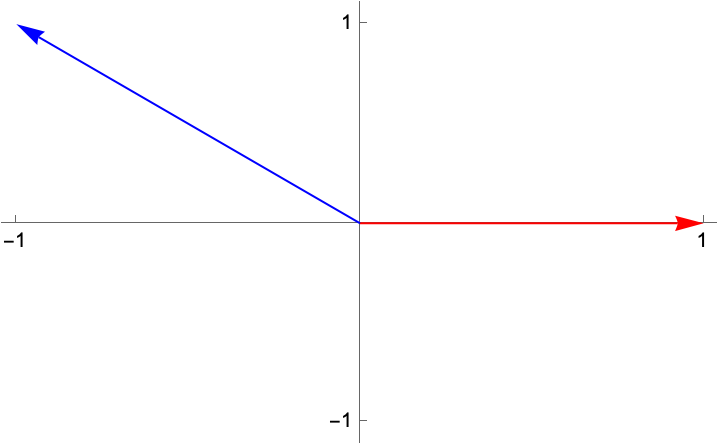
\includegraphics[width=8cm]{misc/horizontalshear.png}
        \caption{Shear of $\Vec{e_1}, \Vec{e_2}$ towards left}
    \end{figure}
    
    \item $A = \twobytwomatrix{0}{-1}{1}{0}$ 
    
    $T(\Vec{e_1}) = \twodmatrix{1}{0} \twobytwomatrix{0}{-1}{1}{0} = \twodmatrix{0}{1}, T(\Vec{e_2}) = \twodmatrix{0}{1} \twobytwomatrix{0}{-1}{1}{0} = \twodmatrix{-1}{0}$
    
    \begin{figure}[!ht]
        \centering
        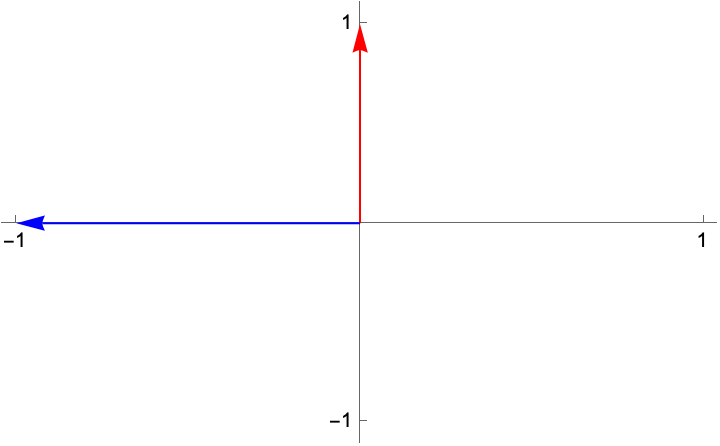
\includegraphics[width=8cm]{misc/rotationaboutorigin.png}
        \caption{Rotation counter-clockwise of $\Vec{e_1}, \Vec{e_2}$ about the origin}
    \end{figure}
\end{itemize}

In these transformations, finding the effect on the standard basis vectors is typically quite simple, while finding the transformation for any random vector can be quite difficult. So, we can instead use the rules of linear transformations to find the effect on any vector in terms of its ratio to the standard basis vectors.

\subsubsection{A Quick Look at Projections}

If a plane $P$ passes through the origin in $\real^n$, any vector $\Vec{x} \in \real^n$ can be written as $\Vec{x}^{\parallel} + \Vec{x}^{\perp}$, where $\Vec{x}^{\parallel}$ is a vector \textit{in the plane} $P$ and $\Vec{x}^{\perp}$ is a vector \textit{perpendicular} to $P$. This can be defined as a linear transformation $\text{proj}_P:\real^n \to \real^n = \text{proj}_P(\Vec{x}) = \Vec{x}^{\parallel}$

\section{Unit 2}
\subsection{Images and Kernels}

For a matrix $A$, we can define the following (useful) subsets:

\begin{itemize}
    \item \textbf{kernel:} aka null space, written ker$(A)$, is the set of vectors $\Vec{x}$ where $A\Vec{x} = \Vec{0}$.
    
    \item \textbf{image:} written im$(A)$, the set of vectors $\Vec{y}$ where $\Vec{y} = A\Vec{x}$. This is more commonly known as the "range" for functions.
\end{itemize}

You can solve for ker$(A)$ by simply augmenting $A$ by $\Vec{0}$.

\subsubsection{Rank-Nullity Theorem}

A useful pattern to keep in mind is that the rank of an rref matrix is equal to the dimension of the image, and the number of free columns in the rref matrix is equal to the dimension of the kernel.

This pattern leads to what is called the \textbf{Rank-Nullity Theorem}.

\subsection{Matrix Algebra}

Similarly to processes described earlier for performing algebraic operations between vectors and vectors, as well as vectors and matrices, it is also possible to perform a number of operations between matrices. However, there are some very specific limitations and rules that must be followed that can make said operations rather unintuitive if viewed as purely extensions of the operations performed between numbers, for instance.

\begin{itemize}
    \item \textbf{Matrix times scalar}
    
    Multiplying a matrix $A$ times a scalar $k$ is very similar to multiplying a vector times a scalar:
    
    \begin{equation}
        \begin{split}
            kA &= k\twobytwomatrix{A_{1a}}{A_{2a}}{A_{1b}}{A_{2b}}\\
            &= \twobytwomatrix{k A_{1a}}{k A_{2a}}{k A_{1b}}{k A_{2b}}\\
        \end{split}
    \end{equation}
    
    \item \textbf{Matrix plus matrix}
    
    Adding together two matrices (say $A$, a $n$ x $m$, and $B$, a $p$ x $q$) requires certain restrictions on the dimensions of the affected matrices, just as in vector addition. In this case, $n=p$ and $m=q$:
    
    \begin{equation}
        \begin{split}
            A + B &= \begin{bmatrix}
            A_{1a} & A_{2a} & A_{3a}\\
            A_{1b} & A_{2b} & A_{3b}\\
            \end{bmatrix} + \begin{bmatrix}
            B_{1a} & B_{2a} & B_{3a}\\
            B_{1b} & B_{2b} & B_{3b}\\
            \end{bmatrix}\\
            &= \begin{bmatrix}
            A_{1a}+B_{1a} & A_{2a}+B_{2a} & A_{3a}+B_{3a}\\
            A_{1b}+B_{1b} & A_{2b}+B_{2b} & A_{3b}+B_{3b}\\
            \end{bmatrix}
        \end{split}
    \end{equation}
    \item \textbf{Matrix times matrix}
    
    In order to multiply two matrices (say $A$, a $n$ x $m$, and $B$, a $p$ x $q$), another set of restrictions apply, that may be a little trickier to interpret. Say you're finding $AB$; here, $m = p$, and the resulting matrix is an $n$ x $q$ matrix. 
    
    When multiplying two matrices, you can imagine the first matrix being multiplied by each of the columns of the second matrix, treating each column as a vector. The result of each vector-matrix multiplication becomes the corresponding column of the resulting matrix. Given these steps, the above restrictions should hopefully make more intuitive sense.
    
    It should also be clear from these steps that \textbf{multiplying matrices is not commutative;}
    
    \begin{equation}
        \begin{split}
            &A = \begin{bmatrix}
            1 & 0 & 2 \\
            2 & -2 & 1 \\
            3 & 1 & 0 \\
            \end{bmatrix}\\
            &B = \begin{bmatrix}
            -1 & 3\\
            2 & 0\\
            1 & 1\\
            \end{bmatrix} = \begin{bmatrix}
            \Vec{b_1} & \vec{b_2}\\
            \end{bmatrix}\\
            AB &= \begin{bmatrix}
            A\Vec{b_1} & A\Vec{b_2}\\
            \end{bmatrix}\\
            &= \begin{bmatrix}
                (-1*2+2*0+1*2) & (3*1 + 0*0 + 1*2) \\
                ... & ...\\
                ... & ...\\
            \end{bmatrix}\\
            &= \begin{bmatrix}
                1 & 5\\
                -5 & 7\\
                -2 & 9\\
            \end{bmatrix}
        \end{split}
    \end{equation}
    
    Doing $BA$, on the other hand, would result in a $2$ x $3$ matrix, which, naturally, would not be equal to the product of $AB$.
    
    \item \textbf{Identity Matrix}
    
    While not exactly an algebraic operation, its important to note that the notation $I$ is often used to denote the \textbf{identity matrix}, a matrix such that $AI = A$. $I$ is essentially a rref matrix with the same number of leading ones as columns. Example:
    
    \[
    I_{2} = \begin{bmatrix}
    1 & 0\\
    0 & 1\\
    \end{bmatrix}
    \]
    
    \item \textbf{Solving for a matrix given its product}
    
    If you are given a matrix $A$ and the product of $A$ with an unknown matrix $B$, you can find $B$ fairly easily using a similar idea as discussed above; by treating each column of $B$ as a vector.
    
    \begin{equation}
    \begin{split}
        AB = \begin{bmatrix}
        -1 & 0 \\
        4 & 5 \\
        0 & 1\\
        \end{bmatrix}B &= \begin{bmatrix}
        -1 & -1 & 0\\
        9 & -1 & -10\\
        1 & -1 & -2\\
        \end{bmatrix}\\
    \end{split}
    \end{equation}
    
    Treating each column of $B$ as a vector ($\vec{b_1}$, etc), we can write the product of each column of $B$ equal to the corresponding column of the product of $A$ and $B$:
    
    \begin{equation}
    \begin{split}
        \vec{b_1}A = \begin{bmatrix}
        -1\\
        9\\
        1\\
        \end{bmatrix}, ...
        \end{split}
    \end{equation}
    
    Finding the vector that multiplies to a matrix to produce a given vector has already been discussed above, so the steps from here (creating an augmented matrix and solving for each component of $\vec{b_n}$) should be clear. However, we can make the work a little easier by simply creating an augmented matrix of $A$ augmented by the product of $AB$:
    
    \begin{equation}
        \begin{split}
             \begin{array}[t][{@{}cc|ccc@{}}]
                 -1 & 0 & -1 & -1 & 0 \\
                 4 & 5 & 9 & -1 & -10 \\
                 0 & 1 & 1 & -1 & -2 \\
                \end{array}\
        \end{split}
    \end{equation}
    
    All row operations to the left hand side of this matrix would be the same no matter the augmented side, so this technique should (hopefully) seem intuitively correct.
\end{itemize}

\subsection{Compositions}

Recall that we can describe a linear transformation $T(\vec{x})$ as a matrix $A$ times the vector $\vec{x}$. However, what if we want to perform two (or more!) linear transformations, one after another? Rather than simply performing said linear transformations one after another, we can use the concept of \textbf{compositions}.

For instance, say we want $T$ composed with $S$. This can be written as follows, given $T(\vec{x}) = A\vec{x}$ and $S(\vec{x}) = B\vec{x}$:

\begin{equation}
    \begin{split}
        T \circ S &= T(S(\vec{x}))\\
        &= T(B\vec{x})\\
        &= A(B\vec{x})\\
    \end{split}
\end{equation}

This composition, just like the functions is composes, is linear. This can be proved using aforementioned definitions, but should also make intuitive sense. 

Another common question is how to find the single matrix, say $C$, that induces the composition. As shown above, a composition is simply a vector multiplied by a number of matrices, so we can find $C$ by simply multiplying the matrices involved (in this case, $A$ and $B$) using the method described earlier.

Note that, since this is essentially just matrix-matrix multiplication, \textbf{order matters}.

\subsubsection{Transformation Inverses}

Given a particular transformation $\vec{y} = T(\vec{x})$, we know we can describe it as $\vec{y}=A\vec{x}$. However, it is very helpful to be able to describe its inverse, $T^{-1}(\vec{x}) = S(\vec{y}) = \vec{x}$. By a natural extension, we should be able to find a matrix $B$ such that $B \vec{y} = \vec{x}$. Below will describe strategies for finding $B$ for a number of transformations, and later how to generalize said strategies to any matrix $A$.

First, let's look at a number of common linear transformations, and how to determine their inverses; if possible.

\begin{itemize}
    \item \textbf{Reflections}
    
    \[
    T(\vec{x}) = ref_L(\vec{x})
    \]
    
    How do we reflect a vector back over to where it started? Well, as the question almost answers by itself, you simply reflect it again. As such, we can say $T^{-1} = T$.
    
    \item \textbf{Rotations}
    
    \[
    T(\vec{x}) = rot(\vec{x})
    \]
    
    Say our transformation rotates a vector $\vec{x}$ by an angle $\Theta$ clockwise. To invert this, we can simply rotate it counterclockwise by $\Theta$, or, equivalently, clockwise by $-\Theta$.
    
    \item \textbf{Projections}
    
    \[
    T(\vec{x}) = proj_L(\vec{x})
    \]
    
    How can we invert a projection? Simply put: we can't! When a vector $\vec{x}$ is projected onto a line $L$, for instance, we lose information about the original $\vec{x}$, and thus have no way of returning to $\vec{x}$. Another way to interpret this is that $T(\vec{x})$ for any $\vec{x} \perp L$ equals $\vec{0}$, and thus it is impossible to go backwards to find any individual $\vec{x}$.
\end{itemize}

From these few examples, we can generalize the following: a transformation $T: \real^m \to \real^n$ is only invertible if for all \textit{outputs} $\vec{y} \in \real^n$ there exist a $\vec{x} \in \real^m$ such that $T(\vec{x}) = \vec{y}$ and $\vec{x}$ is unique.

We can think about this a little differently by considering $A$ such that $T(\vec{x})=A\vec{x} = \vec{y}$. Given our definition above, $A\vec{x}=\vec{y}$ must be consistent for any $\vec{y}$ if $T$ is invertible. As such, we can say that rref$(A)$ must have a leading one in each \textit{row}.

Further, we also require that $A\vec{x}=\vec{y}$ has a unique solution, so rref$(A)$ must also have a leading one in each \textit{column}. 

The only way that this is possible, to begin with, is that the number of columns of $A$ equals to the number of rows of $A$, and by extension, rref$(A) = I$. In other words, the matrix must be square.

\subsubsection{Inverting a Matrix}

As seen earlier in Unit 1, we can say that a transformation $T(\vec{x}) = A\vec{x} = \begin{bmatrix}
T(\vec{e_1}) & T(\vec{e_2})
\end{bmatrix}\vec{x}$. To find the inverse of $A$ ($A^{-1}$), we can say that $A^{-1} = \begin{bmatrix}T^{-1}(\vec{e_1}) & T^{-1}(\vec{e_2})\end{bmatrix}$.

We can say that $\vec{c_n} = T^{-1}(\vec{e_n})$, so $T(\vec{c_n}) = \vec{e_n}$. Thus, we can say that each $n$th column of matrix $A$ times some $\vec{c_n}$ equals $\vec{e_n}$. To find each $\vec{c_n}$ (ie, find each column of $A^{-1}$), we can therefore augment $A$ by the corresponding number of unit vectors; or, in other words, $I_n$.

For example, to invert $\begin{bmatrix} 3 & 2\\
7 & 5\\
\end{bmatrix}$, we write:

\begin{equation}
    \begin{split}
        \begin{array}[t][{@{}cc|cc@{}}]
             3 & 2 & 1 & 0\\
             7 & 5 & 0 & 1\\
            \end{array}&\\
    &=\begin{array}[t][{@{}cc|cc@{}}]
             1 & 0 & \vec{c_1} & \vec{c_2}\\
             0 & 1 & | & |\\
        \end{array}\\
    &=\begin{array}[t][{@{}c|c@{}}]
             I & A^{-1}\\
        \end{array}\\
    \end{split}
\end{equation}

\subsection{Bases and Coordinates}

\subsubsection{Introduction}
% this part is really wordy, maybe fix?
To understand the use of bases in linear algebra, consider the standard basis vectors, $\vec{e_1}, \vec{e_2}, ..., \vec{e_n}$. Any vectors in $R^n$ can thus be rewritten as a combination of these standard vectors ($c_1\vec{e_1} + c_2\vec{e_2} + ... + c_n\vec{e_n}$). However, consider a situation in which, say, "movements" are restricted to only a particular set of vectors (say $\vec{v_1}$ and $\vec{v_2}$) that aren't the standard basis vectors. 

While you can write these vectors, or any combinations of these vectors, as a combination of standard basis vectors, it can be easier to call these vectors as a new set of "basis vectors". We define this as $\mathfrak{B} = \{\vec{v_1}, \vec{v_2}\}$, ie $\mathfrak{B}$ is a basis of $\real^2$.

When writing about vectors in basis $\mathfrak{B}$, we use the notation $[y]_{\mathfrak{B}} = \begin{bmatrix}
    c_1\\
    c_2\\
\end{bmatrix}$ to indicate the coordinates of $\Vec{y}$ in the $\mathfrak{B}$ basis. This vector can thus, by extension, be represented as a linear transformation of the vectors in the basis $\mathfrak{B}$.

\subsubsection{Changing Bases}

To change a vector from one base to another, we can find a matrix $S$ such that $S[\vec{x}]_{\mathfrak{B}} = \vec{x}$, where $S$ is typically called the "change of basis matrix", in this case, changing base from $\mathfrak{B}$ to the standard basis.

Finding $S$ is fairly straightforward. We know that $S$ times each vector in $\mathfrak{B}$ must equal the corresponding standard basis vector, so we can write $S\vec{v_1} = \vec{e_1}$, $S\vec{v_2} = \vec{e_2}$, and so on. Therefore, $S$ simply equals the matrix of the vectors in $\mathfrak{B}$, ie $S = \begin{bmatrix}
    | & | & |\\
    \vec{v_1} & \vec{v_2} & ...\\
    | & | & |\\
\end{bmatrix}$.

To extend this, since we can say that $S[\vec{x}]_{\mathfrak{B}} = \vec{x}$, we can inversely say that $[\vec{x}_{\mathfrak{B}}] = S^{-1}\vec{x}$, so to find the matrix that changes bases in the opposite direction, we simply find the inverse of $S$. From here, this same rationale can be extended transform between any two bases in the same $\real^{n}$.

\subsubsection{Application to Transformations}

As noted earlier, we can define a linear transformation as a matrix $A$ such that $T(\vec{x}) = A\vec{x}$. With the added knowledge of bases, we can often more easily find the matrix of a transformation by carefully picking a basis for the transformation which makes the matrix easier to find.

To demonstrate this, take a transformation $T$ that projects vectors in $\real^{3}$ onto the plane $P$ defined by $3x_1+2x_2-5x_3=0$. To find a matrix $A$ such that $T(\vec{x}) = A\vec{x}$, we can create a basis $\mathfrak{B}$ of $R^{3}$ using vectors that make $A$ easy to compute.


For this particular case, we can define $\mathfrak{B} = \{\vec{v_1}, \vec{v_2}, \vec{v_3}\}$, where:

\begin{itemize}
    \item $\vec{v_1} = \begin{bmatrix}
        3\\
        2\\
        -5
    \end{bmatrix}$, since $T(\vec{v_1}) = 0$, as it is perpendicular to $P$

    \item $\vec{v_1} = \begin{bmatrix}
        0\\
        5\\
        2
    \end{bmatrix}$, since $T(\vec{v_2}) = \vec{v_2}$, as it lies along $P$

    \item $\vec{v_1} = \begin{bmatrix}
        5\\
        0\\
        3
    \end{bmatrix}$, since $T(\vec{v_3}) = \vec{v_3}$, as it also lies along $P$
\end{itemize}

To put it in more clear notation, we say that $[T(\vec{v_1})]_{\mathfrak{B}} = \vec{0}$, $[T(\vec{v_2})]_{\mathfrak{B}} = \begin{bmatrix}
0\\
1\\
0\\\end{bmatrix}$, and $[T(\vec{v_3})]_{\mathfrak{B}} = \begin{bmatrix}
    0\\
    0\\
    1\end{bmatrix}$; this step should make sense, as each vector denoted is the corresponding combination of vectors in $\mathfrak{B}$. Here, it should be clear that any vectors that that form a base of $\real^{3}$ could realistically have been used here, but these are clearly easier to work with.

    From here, we can define $B$, such that $B[\vec{v_1}]_{\mathfrak{B}} = [T(\vec{v_1})]_{\mathfrak{B}}$, simply enough as $B = \begin{bmatrix}
        0 & 0 & 0\\
        0 & 1 & 0\\
        0 & 0 & 1\\
    \end{bmatrix}$.

    From the previous section, we showed that $S^{-1}\vec{x} = [\vec{x}]_{\mathfrak{B}}$. Extending that to this linear transformation, we can recap our steps above using a number of matrices, as follows:

    \begin{equation}
        \begin{split}
            T(\vec{x}) &= A\vec{x}\\
            [T(\vec{x})]_{\mathfrak{B}} &= B[\vec{x}]_{\mathfrak{B}}\\
            [T(\vec{x})]_{\mathfrak{B}} &= B\red{S^{-1}}\vec{x}\\
            T(\vec{x})&= \red{S}BS^{-1}\vec{x}\\
            \implies A &= SBS^{-1}\\
        \end{split}
    \end{equation}

The final line above indicates a general process that can be used to find a matrix to represent any linear transformation, and while this process may seem initially more difficult that previously discussed methods, it has many advantages as well.

\subsection{Elementary Matrices}

Throughout these notes, the idea of "Gaussian elimination" and row reduction has been constantly discussed, with the concept of modifying the rows and columns of a matrix through a number of operations. \textbf{Elementary matrices} define matrices that, when multiplied to another matrix, execute these same row operations. These are typically denoted with an $E$.


\subsubsection{Types of Elementary Matrices}

Just as there a set number of possible row operations that we can perform on matrices, there are a corresponding number of elementary matrices that we can define to perform the equivalent transformations.

\begin{itemize}
    \item[\textbf{I}]: Row Interchanges
    
    This type of elementary matrix simply swaps rows of a matrix. For example, for a 2 by 3 matrix:


    \begin{equation}
        \begin{bmatrix}
            0 & 1 \\
            1 & 0\\
        \end{bmatrix} \begin{bmatrix}
            a & b & c\\
            p & q & r\\
        \end{bmatrix} = \begin{bmatrix}
            p & q & r\\
            a & b & c\\
        \end{bmatrix}
    \end{equation}

    The elementary matrix $\begin{bmatrix}
        0 & 1\\
        1 & 0\\
    \end{bmatrix}$ swaps the first and second rows, as shown. It should also be clear that there could be \textit{any number of columns in the matrix on the left}, and the elementary matrix would still perform the same operation.

    Finding the matrix to exchange rows for any dimension of matrix is fairly straightforward, as the matrix will only involve $0$'s and $1$'s in different positions.

    If we were to invert this operation, we can simply use the same elementary matrix again. Thus, in this case, $E = E^{-1}$; this can be verified by manually inverting $E$ as well, by using methods described earlier. 

    \item[\textbf{II}]: Row Multiplication

    To multiply a particular row (or rows) of a matrix by a constant, we can define another fairly simply elementary matrix that involves essentially all $1$'s and $0$'s again, except for the appropriate constant in the appropriate position. For instance, say we want to multiply the second row of the same matrix as above by $3$:

    \begin{equation}
        \begin{bmatrix}
            1 & 0 \\
            0 & 3\\
        \end{bmatrix} \begin{bmatrix}
            a & b & c\\
            p & q & r\\
        \end{bmatrix} =  \begin{bmatrix}
            a & b & c\\
            3p & 3q & 3r\\
        \end{bmatrix}
    \end{equation}

    To invert this operation, we have to divide the appropriate row by the same constant, or, more appropriately, multiply it by the inverse of the constant. Thus, $E^{-1} = E$ but with the constant inverted (fractional).

    \item[\textbf{III}]: Adding Multiples of Rows
    
    Adding a certain number of a row (or rows) to another row (or rows) of a matrix is, often, the most complicated to describe with an elementary matrix. However, with an example, it should hopefully be rather clear; so, to add twice the second row to the first row of a matrix, consider the following:

    \begin{equation}
        \begin{bmatrix}
            1 & 2 \\
            0 & 1\\
        \end{bmatrix} \begin{bmatrix}
            a & b & c\\
            p & q & r\\
        \end{bmatrix} =  \begin{bmatrix}
            a + 2p & b + 2q & c + 2r\\
            p & q & r\\
        \end{bmatrix}
    \end{equation}

    To invert this operation, we have to subtract the constant times the same row from the row involved. In this particular case, $E^{-1} = \begin{bmatrix}
        1 & -2\\
        0 & 1\\
    \end{bmatrix}$.
\end{itemize}

It should be noted that, in all these operations, the elementary matrix was invertible; and not only that, the inverted elementary matrix was also an elementary matrix in its own regard. If we want to invert such a matrix, we can either do so with typical methods (augmenting it by $I$) or by simply finding the logical inverse of the operation that the elementary matrix performs. 

It should be noted that you will often see problems with the following format, for some matrix $A$:

\begin{equation}
    E_5E_4E_3E_2E_1A
\end{equation}

While this may seem scary, since it is a whole lot of matrix-matrix multiplication, once you are able to determine what operation each $E_n$ performs, calculating this should be fairly straightforward. Simply find $A$ after $E_1$'s operations on performed on it, then after $E_2$ is performed on the result of that, etc..

\subsection{Distances}

\section{Unit 3}

\subsection{Curve Fitting}

\subsection{Orthogonality and the Transpose of a Vector}

\subsection{Least Squares, etc.}

\newpage
\section{Summary of Terms}
This course relies \textbf{heavily} on vocabulary. Below is a brief conglomeration (ignore the oxymoron) of these terms.

\subsection{Notation}
    \begin{itemize}
        \item $\real$: real numbers
        \item $\integers$: integers
        \item $\naturals$: natural numbers
        \item $\real^n$: the $n$th real dimension
        \item ${...}$: set
        \item $\in$: "is in"
        \item $\exists$: "exists"
        \item $\therefore$: "therefore"
        \item $\Vec{u}$: vector named "$u$"
        \item $\Vec{0}$: "0 vector", vector of any dimension with all $0$'s
        \item $f: A \to B$: "a function $f$ takes inputs of dimension $A$ and returns outputs of dimensions $B$"
        \item $T \circ S$: "$T$ composed with $S$"
        \item  \item $\mathfrak{B}, \mathfrak{C}, ...$: a basis of some $\real^n$
        \item $[\vec{x}]_{\mathfrak{B}}$ a vector $\vec{x}$ represented in base $\mathfrak{B}$
        \item $E$: some elementary matrix
       \item $A^{-1}$: the inverse of a matrix $A$
    \end{itemize}
\subsection{Vocabulary}
    \begin{itemize}
        \item \textbf{rref}: 
        \begin{itemize}
            \item "reduced row echelon form"
            \item a matrix (representing a system of linear equations) that has been manipulated to have the following properties:
            \begin{itemize}
                \item the first non-zero in each row is a \textit{leading 1}, with 0's above and below
                \item the leading 1 in any row is to the right and below the leading 1 above it
                \item rows with all 0's are at the bottom (\textit{this is purely convention})
            \end{itemize}
        \end{itemize}
        \item \textbf{rank}: the number of leading 1's in the \textit{rref} of a matrix
        \item \textbf{linear combination}: a sum of multiples of a number of vectors.
        
        eg, $c_1 \Vec{v_1} + c_2 \Vec{v_2}$ would be a linear combination of $\Vec{v_1}$ and $\Vec{v_2}$.
        
        \item \textbf{span}: all possible \textit{linear combinations} of some vectors, denoted as span($\Vec{v_1}, \Vec{v_2}$)
        
        \item \textbf{linear relation}: an equation of the form $c_1 \Vec{v_1} + c_2 \Vec{v_2} + ... + c_n \Vec{v_n} = \Vec{0}$ for the vectors $\Vec{v_1}, \Vec{v_2}, ..., \Vec{v_n}$.
        
        \begin{itemize}
            \item if the only way this relation holds true are when all $c_n = 0$, then this is called a \textbf{trivial linear relation}
            \item if at least one $c_n \neq 0$, then this is called a \textbf{nontrivial linear relation}
        \end{itemize}
        
        \item \textbf{linear (in)dependence}: 
        \begin{itemize}
            \item a set of vectors are \textbf{linearly independent} if the only \textit{linear relation} between them is the \textit{trivial} one
            \item a set of vectors are \textbf{linearly dependent} if there exists a \textit{linear relation} between them that is \textit{nontrivial}
        \end{itemize}
        
        \item \textbf{basis}: the minimal set of vectors in a subspace needed to span that subspace. By extension, it can be said that a set of vectors $x$ is the basis of a subspace $V$ if:
        
        \begin{itemize}
            \item $x$ \textit{spans} $V$
            \item the vectors in $x$ are \textit{linearly independent}
        \end{itemize}
        
        \item \textbf{dimension}: the number of vectors in a \textit{basis} of a \textit{span}
        
        \item \textbf{subspace}: a non-empty set of vectors in $\real^n$ that can be denoted as a span of vectors. A subset $V$ of $\real^n$ can be qualified as a subspace if:
        
        \begin{itemize}
            \item the subset is \textit{closed under scalar multiplication}: for any $\Vec{u} \in V$, $k \Vec{u} \in V$ for any scalar $k\in\real$
            \item the subset is \textit{closed under addition}: for any $\Vec{u}, \Vec{w} \in V$, $\Vec{u} + \Vec{w} \in V$
        \end{itemize}
        
        \item \textbf{standard basis}: the set of unit vectors forming a basis of $\real^n$. These are denoted by $\Vec{e_i}$, with $i$ ranging from $1$ to $n$.
        
        For example, in $\real^n$, the standard basis vectors are $\Vec{e_1} = \twodmatrix{1}{0}, \Vec{e_2} = \twodmatrix{0}{1}$.
        
        \item \textbf{matrix multiplication}: the process of multiplying a vector $\Vec{x}$ by a matrix $A$. There are two ways of visualizing this process:
        
        \begin{itemize}
            \item \textit{column view}:
            
            $$A \Vec{x} = \begin{bmatrix}
            | &| & &|\\
            \Vec{c_1} &\Vec{c_2} &... &\Vec{c_n}\\
            | &| & &|\\
            \end{bmatrix}\Vec{x} = \begin{bmatrix}
            x_1\\
            x_2\\
            ...\\
            x_n
            \end{bmatrix} = x_1 \Vec{c_1} + x_2 \Vec{c_2} + ... + x_n \Vec{c_n}
            $$
            
            In this case, each column of $A$ is treated as a vector, and multiplied by each component of $\Vec{x}$.
        
        \item \textit{row view}:

        $$A\Vec{x} = \begin{bmatrix}
        &- & \Vec{r_1} &-\\
        &- & \Vec{r_2} &-\\
        & & ... &\\
        &- & \Vec{r_m} &-\\
        \end{bmatrix}\Vec{x}=\begin{bmatrix}
        \Vec{r_1} \cdot \Vec{x}\\
        \Vec{r_2} \cdot \Vec{x}\\
        ...\\
        \Vec{r_m} \cdot \Vec{x}\\
        \end{bmatrix}$$
        
        In this case, each row of $A$ is treated as a vector, and the \textit{dot product} of $\Vec{x}$ and each row becomes the row of the resulting vector.
        
        \end{itemize}
        
        Note that in either view, the answers are equivalent, and using one view or the other simply helps make particular operations easier.
        
        \item \textbf{linear transformations}: a function $T: \real^n \to \real^m$ that has the following two properties:
        \begin{itemize}
            \item \textbf{preserves vector addition}: $T(\Vec{x} + \Vec{y}) = T(\Vec{x}) + T(\Vec{y}), \Vec{x}, \Vec{y} \in \real^n$
            \item \textbf{preserves scalar multiplication}: $T(c \Vec{x}) = c T(\Vec{x}), \Vec{x}\in\real^n, c\in\real$
        \end{itemize}
        
        \item \textbf{kernel}: the set of vectors $\Vec{x}$ such that $A\Vec{x} = \Vec{0}$, denoted by ker$(A)$
        
        \item \textbf{image}: the set of vectors $\Vec{y}$ such that $\Vec{y} = A\Vec{x}$ for some vector $\Vec{x}$, denoted by im$(A)$; also known as the \textit{range}.
        
        \item \textbf{rank-nullity theorem}: "the \textit{rank} of an rref matrix is equal to the dimension of the \textit{image}, and the \textit{number of free columns} is equal to the dimension of the \textit{kernel}".
        
        \item \textbf{identity matrix}: denoted $I_n$ for some integer $n$, a matrix of $n$ rows and $n$ columns of the format $\begin{bmatrix}
        1 & 0 & ... & 0\\
        0 & 1 & ... & 0\\
        0 & 0 & ... & 0 \\
        | & | & ... & 1 \\
        \end{bmatrix}$

        \item \textbf{composition}: a number of transformations performed in a particular order. For instance, given the linear transformations $T$ and $S$ and a vector $\vec{x}$, we can denote performing $S$ and then $T$ on $\vec{x}$ by saying:
        
        $$T \circ S = T(S(\vec{x}))$$

        Note that "$\circ$" is read as "$T$ composed with $S$".

        Its important to note that it is \textit{not necessarily true} that $S \circ T = T \circ S$.

        \item \textbf{inverses}: just as the inverse of a function, the inverse of a matrix is a matrix that undoes the operations of a matrix. More information can be found above, but to invert a matrix you can simply augment it by the corresponding $I_n$.
        
        A matrix, $A$, is only invertible if:

        \begin{itemize}
            \item $A$ is square (\textit{number of rows = number of} columns)
            \item rref$(A) = I$
        \end{itemize}

        This second requirement does in fact incorporate the first, but it is helpful to explicitly state the first as it can make determining if certain matrices are invertible or not very simple.

        \item \textbf{elementary matrix}: a matrix that performs a row operation on a matrix. They are typically denoted $E$, are always invertible, and their inverses are always elementary matrices as well. Also, by extension of always being invertible, they are, of course, always square.
        
        
    \end{itemize}

\end{document}